\documentclass[twocolumn,twoside]{base/ajstd}

\newcolumntype{Y}{>{\raggedright\arraybackslash}X}

% Article information (authors ignore)
\articleinformation{Vol xx, No x, 2026, xx--xx}
\articleinformationtruncated{xx(x): xx--xx}
\articledoi{10.29037/ajstd.xxx}
\articletype{RESEARCH ARTICLE}
\submitted{\enspace 16 May 2026} \revised{\enspace 16 June 2026} \accepted{\enspace 16 June 2026}

% Article title
\title{TinyML Smart Plug for Complementary Protection Against Progressive Fire-Inducing Electrical Faults in Residential Circuits}

% Author(s)
\author[1,\mbox{*}]{Francis M. Pe\~{n}a}
\author[1]{Jett M. Lumabi}
\author[1]{Alex A. Alferez}
\author[1]{Referendo D. Soriano}

\authorheader{Pe\~{n}a et al.}

% Author(s) affiliations
\affil[1]{College of Science, Engineering and Architecture, Ateneo de Naga University, Naga City 4400, Philippines}

% Corresponding author
\affil[$\mbox{*}$]{Corresponding author: \href{mailto:fpenaofficial@gmail.com}{fpenaofficial@gmail.com}}

% Abstract
\abstract{Localized plug-socket faults can progress to fire hazards through sustained overload, degraded-contact heating, and load-limited series arcing before conventional upstream protection responds. This paper presents a TinyML-enabled smart plug for complementary socket-level intervention in 230 V residential circuits. The prototype integrates custom current sensing, anti-aliasing and digitization, socket-temperature estimation from a contact-region thermistor, embedded Random Forest arc inference, deterministic overload and heating logic, event logging, and latched relay disconnection. Current frames were sampled at 27 kHz and converted to conduction-gap, baseline-departure, and spectral-disturbance features with load-context fields. Controlled validation gave mean absolute errors of 0.178 A for current and 1.02\degree C for temperature sensing. In overload tests, warning occurred in all heavy-load trials, while the sustained 17.30 A case tripped after 61.3 s. Degraded contacts heated faster than normal contacts under matched loads; the most severe protection trial tripped at an estimated 40.0\degree C while the reference terminal reached 56.0\degree C. Across 200 arc and normal trials, the deployed model-plus-firmware logic achieved 97.50\% accuracy, 98.97\% precision, 96.00\% recall, and 97.46\% F1-score. Results support prototype-scale feasibility for localized protective intervention, with broader field validation still required.}

% Keywords
\keywords{\texorpdfstring{degraded contacts;\\embedded inference;\\series arcing;\\thermal estimation;\\waveform features}{degraded contacts; embedded inference; series arcing; thermal estimation; waveform features}}

% PDF metadata (authors ignore)
\makeatletter
	\hypersetup{%
		pdftitle={\@title},%
		pdfauthor={\authorheader},%
    	pdfkeywords={\keywords},%
    	pdfsubject={\abstract}%
    }
\makeatother

\makeatletter
\def\MT@warn@unknown{}
\makeatother

\begin{document}

\setcounter{page}{1}

\maketitle
\thispagestyle{firststyle}
\linenumbers

\section{INTRODUCTION}

Electrical fires remain a persistent residential safety problem because multiple failure mechanisms can produce localized heating, arcing, or ignition before a simple breaker-level overcurrent condition is apparent \citep{Meng2024ElectricalFires,DaRocha2023ElectricalFireRisk,Taylor2024HomeFireInjuries}. At the outlet level, three fault classes are especially relevant to plug-connected appliances: sustained overload, poor-contact or degraded-contact heating, and load-limited series arcing. Poor plug-socket contact can raise local resistance and temperature, while thermally degraded insulation can support arc tracking at a plug-outlet connection \citep{Zhang2021PoorContact,Li2024PoorContact,Hadziefendic2018ReducedTorque,Okamoto2022ArcTracking}. These mechanisms are local, progressive, and strongly affected by contact condition, load current, materials, and thermal paths.

Conventional branch-circuit protection and certified arc-fault devices remain essential safety layers. However, upstream devices do not directly measure the thermal condition of a specific socket interface, and arc detection is difficult because normal appliances can produce nonlinear current, switching transients, motor noise, and high-frequency components that resemble fault signatures \citep{Lee2000AFCI,Zhao2022SeriesArc,Gong2022SeriesArc,Chen2024LightweightArc}. This motivates a complementary device located at the plug-socket interface, where current waveform behavior, local temperature, and relay intervention can be combined without cloud dependence.

This paper presents a TinyML Smart Plug for complementary socket-level protection against progressive fire-inducing faults in residential circuits. Its contribution is an integrated prototype that combines custom hardware, anti-aliasing and digitization, embedded feature extraction, local load-context and series-arc inference, deterministic overload and heating protection, event logging, and relay-based intervention. The device is evaluated as a controlled-laboratory research prototype, not as a certified replacement for breakers, AFCIs, GFCIs, electrical inspection, or code-compliant wiring.

\section{MATERIALS AND METHODS}

\subsection{Prototype Hardware and Physical Design}

Figure~\ref{fig:system-architecture} summarizes the system architecture. The prototype was implemented as a plug-through 230 V single-phase smart plug. A custom hardware stack integrated the line-side plug, protected outlet, relay switching path, ESP32-S3 controller, current sensing, voltage context sensing, socket-temperature sensing, local indicators, enclosure, and logging interface. Voltage was retained only for waveform acquisition context, mains-state interpretation, and calibration; voltage-trip behavior is outside the scope of this article.

\begin{figure*}[!t]
	\centering
	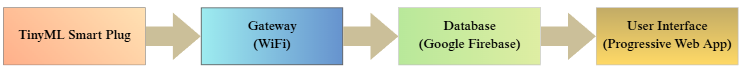
\includegraphics[width=0.86\linewidth]{figures/system_architecture.png}
	\caption{System architecture of the TinyML Smart Plug prototype. Protection decisions are executed locally on the ESP32-S3; cloud logging and the web interface support review, labeling, and monitoring.}
	\label{fig:system-architecture}
\end{figure*}

The current path used an ACS37035 Hall-effect sensor with its analog output routed through an active anti-aliasing stage and an MCP3204 external analog-to-digital converter. The second-order low-pass stage was set near 10 kHz using
\begin{equation}
  f_0=\frac{1}{2\pi\sqrt{R_1R_2C_1C_2}}\approx 9.98\ \mathrm{kHz},
  \label{eq:aaf-cutoff}
\end{equation}
for $R_1=200$ k$\Omega$, $R_2=33$ k$\Omega$, $C_1=470$ pF, and $C_2=82$ pF. The stage conditioned the current waveform before the firmware sampled 512-point frames for arc-feature extraction. A 10 k$\Omega$ NTC thermistor was placed near the plug-side contact region to provide a non-intrusive proxy for local socket heating. The relay was driven through a latched fault path so that a confirmed fault remained disconnected until reset.

\begin{figure}[!t]
	\centering
	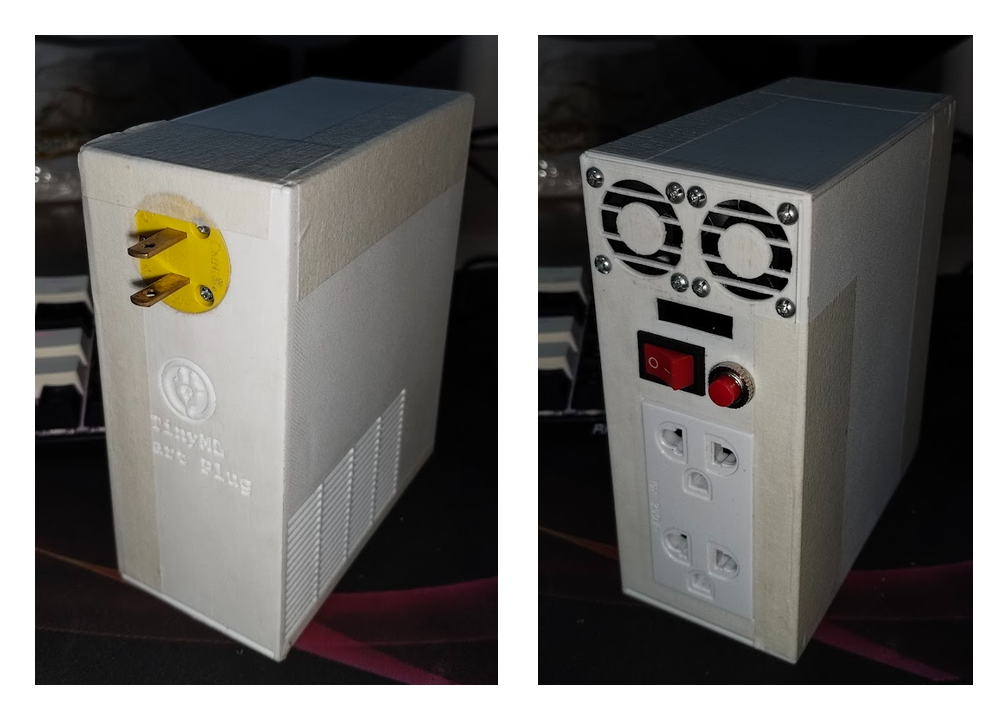
\includegraphics[width=\linewidth]{figures/prototype_enclosure.png}
	\caption{Completed prototype enclosure showing the plug side and protected-outlet side used during bench validation. The enclosure documents the research form factor and is not a certification claim.}
	\label{fig:prototype-enclosure}
\end{figure}

Figure~\ref{fig:prototype-enclosure} shows the enclosed prototype. The physical design considered separation of mains and low-voltage wiring, airflow around internal components, access to the protected outlet, front-panel switching, buzzer and display placement, and repeatability during bench testing. The prototype is a laboratory platform; creepage, clearance, insulation barriers, relay rating, enclosure flame rating, and production manufacturability require separate compliance engineering before practical deployment.

\subsection{Embedded Signal Processing and TinyML Workflow}

The arc-detection path used 512-sample current frames at a 27 kHz target sampling rate with a 256-sample hop. A Hann window was applied before frequency-domain computations to reduce spectral leakage \citep{Harris1978Windows}. The firmware computed a broader set of waveform descriptors for logging and review, but the deployed series-arc Random Forest used six base waveform features: maximum low-current run, zero-dwell ratio, low-current ratio, absolute RMS-current z-score relative to baseline, midband residual ratio, and mid/high-frequency spectral flux. These features were selected to capture interruption, restrike, waveform departure, and spectral disturbance, which are recurring indicators in series-arc studies \citep{Zhao2022SeriesArc,Gong2022SeriesArc,Chen2024LightweightArc,Qi2024SeriesArcELM}.

Two representative deployed features are
\begin{equation}
  L_{\mathrm{ratio}}=\frac{100}{N}\sum_{n=0}^{N-1}\mathbf{1}\!\left(|i_c[n]|\le I_{\mathrm{low}}\right),
  \label{eq:low-current-ratio}
\end{equation}
where $I_{\mathrm{low}}=\max\{0.035,\,0.06\max(I_{\mathrm{rms}},0.10)\}$, and
\begin{equation}
  t_{\mathrm{low,max}}=\frac{1000\,N_{\mathrm{run,max}}}{f_s}.
  \label{eq:max-low-run}
\end{equation}
Here $L_{\mathrm{ratio}}$ expresses the percentage of near-zero-current samples, $i_c[n]$ is the cleaned current sample, $N_{\mathrm{run,max}}$ is the longest low-current run, and $f_s$ is the sampling rate. These equations directly represent the extinction-gap behavior expected in a series arc.

Load context was estimated separately from six current-waveform descriptors and encoded as six one-hot family fields plus a confidence value. The deployed arc model therefore used a 13-input vector: six waveform features and seven context fields. The embedded threshold was 0.4800 for supported known contexts, while unknown contexts used a more conservative threshold of 0.7800 and at least three corroborating feature votes. Random Forest classification was selected because tree ensembles can capture nonlinear feature interactions and can be exported as deterministic embedded code \citep{Breiman2001RandomForests}. This offline-training and on-device-inference workflow follows TinyML practice for constrained microcontrollers, where training remains off-device and inference runs locally at the edge \citep{Ray2021TinyMLIoT,Immonen2022TinyMLMicrocontrollers,Antonini2023TinyML}.

The training workflow used firmware CSV logs from normal, startup, and induced-arc sessions. Arc windows were manually reviewed and labeled because true arc frames were sparse relative to normal load operation. Python scripts cleaned the logs, formed train/validation/test splits, trained the load-context and arc models, generated metric reports, and exported C headers for firmware integration. The final embedded behavior combined model output with a leaky persistence counter before relay tripping, so the reported device behavior represents model-plus-firmware protection rather than a standalone frame classifier.

The final arc data view contained 49,296 logged rows with 283 manually marked arc rows, or about 0.577\% positives. The model-development split used 35,512 training rows, 9,434 validation rows, and 10,268 test rows. This imbalance motivated reporting both frame-level model results and trial-level relay outcomes.

\subsection{Protection Logic and Test Procedures}

Overload and socket-heating protection used deterministic logic because their dominant variables were current, time, and temperature. Series-arc protection used TinyML inference plus persistence logic to reduce nuisance trips from isolated frames. Table~\ref{tab:design-summary} summarizes the implemented functions.

\begin{table}[!t]
  	\centering\footnotesize\sffamily
  	\caption{Implemented hardware, sensing, and protection functions.}
  	\begin{tableminipage}{\linewidth}
    	\begin{tabularx}{\linewidth}{p{0.28\linewidth}YY}
			\toprule
            Block & Implementation & Role in evaluation \\
	    	\midrule
            Current path & ACS37035 module, active anti-aliasing, MCP3204 ADC & RMS current, overload logic, waveform features \\
            Thermal path & 10 k$\Omega$ NTC near plug-side contact region & Socket-heating warning and relay trip estimate \\
            Arc inference & 13-input Random Forest exported to firmware & Series-arc classification with load context \\
            Relay path & Latched relay intervention & Local disconnection after confirmed fault \\
            Logging path & Firmware and web review tools & Dataset collection, manual labeling, validation records \\
            \bottomrule
    	\end{tabularx}
        \label{tab:design-summary}
  	\end{tableminipage}
\end{table}

The heating estimator used a squared current-shape term,
\begin{equation}
  s_I=\left[\operatorname{clamp}\left(\frac{I_{\mathrm{rms}}}{12.0},\,0,\,1.25\right)\right]^2,
  \label{eq:thermal-current-shape}
\end{equation}
and selected the larger of a directly compensated thermistor value and an expected normal socket value:
\begin{equation}
  \begin{aligned}
  T_{\mathrm{socket,est}}=
  \operatorname{clamp}\{&\max(T_{\mathrm{NTC}}+\Delta T_{\mathrm{meas}},\\
  &T_a+\Delta T_{\mathrm{normal}}),-20,125\}.
  \end{aligned}
  \label{eq:socket-estimate}
\end{equation}
In (\ref{eq:thermal-current-shape}) and (\ref{eq:socket-estimate}), $T_a$ is the tracked baseline temperature, $\Delta T_{\mathrm{normal}}$ is the filtered normal rise expected from load current, and $\Delta T_{\mathrm{meas}}=0.30+1.20s_I$ when a load is active. Socket-heating warning begins at 39.0\degree C, clears below 38.6\degree C, and trips at $T_{\mathrm{socket,est}}\geq 40.0\degree C$.

Overload persistence and arc persistence were expressed as leaky counters:
\begin{equation}
  S_{\mathrm{OL}}[k]=
  \begin{cases}
  \min(6,S_{\mathrm{OL}}[k-1]+1), & I_{\mathrm{avg}}\geq14.5\ \mathrm{A},\\
  \max(0,S_{\mathrm{OL}}[k-1]-1), & I_{\mathrm{avg}}\leq14.1\ \mathrm{A},
  \end{cases}
  \label{eq:overload-counter}
\end{equation}
updated every 10 s with relay trip at $S_{\mathrm{OL}}=6$, and
\begin{equation}
  C_{\mathrm{arc}}[k]=
  \begin{cases}
  \min(16,C_{\mathrm{arc}}[k-1]+2), & \hat{y}_{\mathrm{arc}}=1,\\
  \max(0,C_{\mathrm{arc}}[k-1]-6), & \hat{y}_{\mathrm{arc}}=0,
  \end{cases}
  \label{eq:arc-counter}
\end{equation}
with relay trip at $C_{\mathrm{arc}}\geq 8$. The arc counter required repeated positive frames and decayed quickly when inference returned to normal.

Figure~\ref{fig:test-setups} shows the physical test setups retained for the journal article. Overload trials used high-power load combinations to verify warning and sustained-trip behavior. Socket-heating tests compared normal and intentionally degraded contacts under matched load cases, recording device temperature, estimated socket temperature, infrared terminal temperature, relay state, and elapsed time. Series-arc trials used a controlled series interruption platform with appliance loads; relay trip was the positive prototype response and an induced series arc was the positive ground-truth condition.

\begin{figure*}[!t]
	\centering
	\begin{subfigure}[t]{0.48\linewidth}
		\centering
		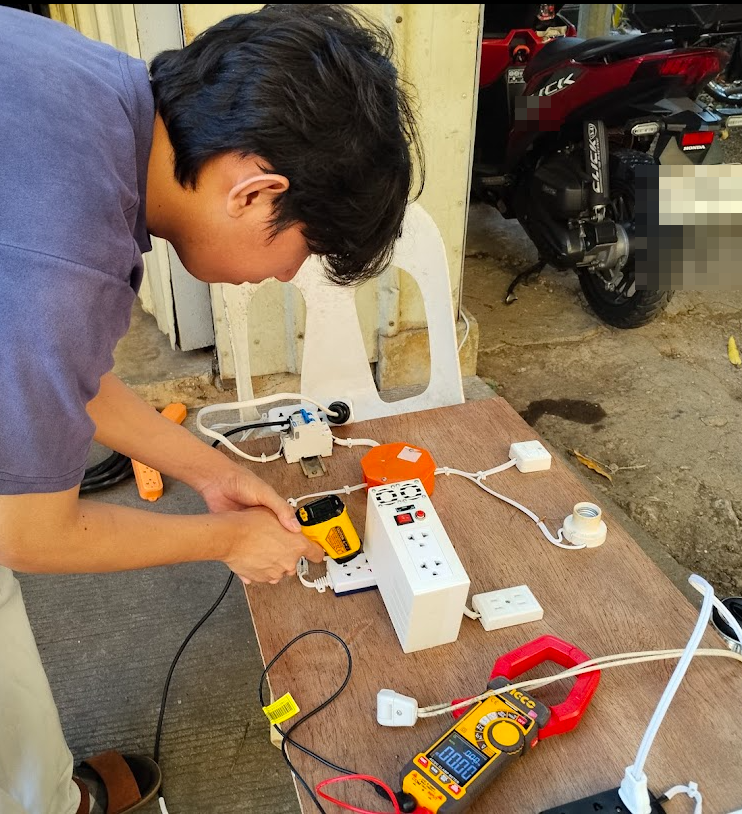
\includegraphics[height=1.7in,keepaspectratio]{figures/socket_heating_setup_blurred.png}
		\caption{Socket-heating validation}
	\end{subfigure}
	\hfill
	\begin{subfigure}[t]{0.48\linewidth}
		\centering
		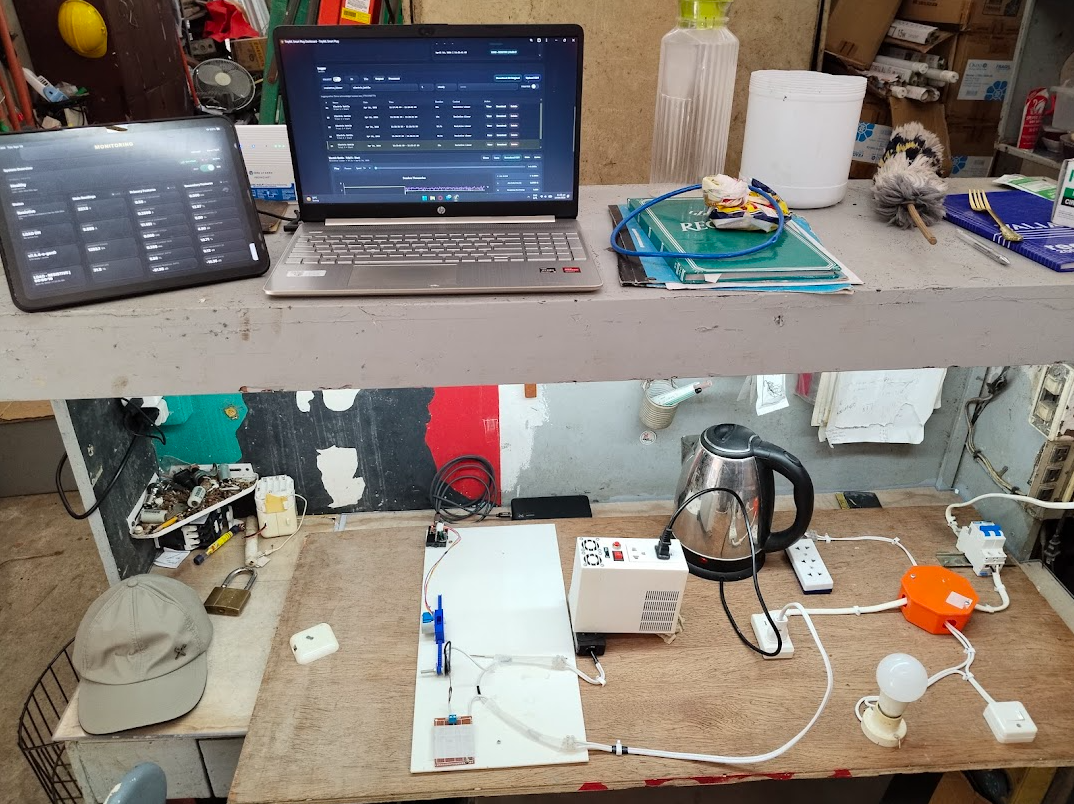
\includegraphics[height=1.7in,keepaspectratio]{figures/series_arc_setup.png}
		\caption{Series-arc validation}
	\end{subfigure}
	\caption{Representative bench setups for contact-heating and series-arc evaluation. The smart plug was placed in the load path so that current, temperature, relay state, and event logs were captured by the same embedded system used for protection.}
	\label{fig:test-setups}
\end{figure*}

Classification performance was computed using accuracy, precision, recall, and F1-score from trial-level true-positive, false-positive, true-negative, and false-negative outcomes. The positive class was a relay trip during an arcing event. Sensor validation used mean absolute error against reference instruments.

\section{RESULTS}

Sensor validation supported the protection decisions used in the prototype. The calibrated current channel had a mean absolute error of 0.178 A, and the thermistor channel had a mean absolute error of 1.02\degree C at the sensor measurement point. The voltage channel produced 3.910 V mean absolute error and was retained for context and logging, but voltage-protection behavior is not reported here because the article focuses on fire-inducing socket faults.

The overload evaluation in Table~\ref{tab:overload-results} shows the intended separation between warning and relay disconnection. Trials with mean currents from 12.33 A to 14.42 A produced warnings but did not trip, even when peaks approached or exceeded 14.5 A. The relay opened only in Trial 4, where the mean current was 17.30 A and the 61.3 s latency agreed with the approximately 60 s persistence design.

\begin{table}[!b]
  	\centering\footnotesize\sffamily
  	\caption{Overload protection results.}
  	\begin{tableminipage}{\linewidth}
    	\begin{tabularx}{\linewidth}{p{0.10\linewidth}p{0.38\linewidth}YYY}
			\toprule
            Trial & Load setup & Mean A & Peak A & Relay \\
	    	\midrule
            1 & Kettle + water heater & 12.87 & 14.85 & No \\
            2 & Two kettles & 12.33 & 13.63 & No \\
            3 & Kettle + water heater & 13.36 & 14.86 & No \\
            4 & Kettle + water heater + two lamps & 17.30 & 19.73 & Yes, 61.3 s \\
            5 & Kettle + water heater + one lamp & 14.42 & 16.23 & No \\
            \bottomrule
    	\end{tabularx}
        \label{tab:overload-results}
  	\end{tableminipage}
\end{table}

Socket-heating validation showed that current magnitude alone was insufficient to describe outlet risk. Table~\ref{tab:heating-results} summarizes the protection trials under normal and corroded contacts. At approximately 9 A, the corroded socket reached the 38.2\degree C device-temperature marker in 48 min, compared with 100 min for the normal socket. At approximately 11 A, the corroded case reached the same marker in 7 min, compared with 54 min for the normal socket. In the most severe corroded case, the estimated socket temperature reached the 40.0\degree C trip threshold after 5 min while the infrared terminal reference reached 56.0\degree C.

\begin{table*}[!t]
  	\centering\footnotesize\sffamily
  	\setlength{\tabcolsep}{3pt}
  	\caption{Socket-heating protection validation. Times are in minutes; dash indicates that the threshold was not reached before the end of the trial.}
  	\begin{tableminipage}{\linewidth}
    	\begin{tabularx}{\linewidth}{p{0.22\linewidth}p{0.09\linewidth}p{0.07\linewidth}p{0.11\linewidth}p{0.09\linewidth}p{0.10\linewidth}p{0.08\linewidth}p{0.06\linewidth}}
			\toprule
            Load case & Socket & Mean A & Dev. 38.2\degree C & Est. 40\degree C & Est. temp. & IR temp. & Relay \\
	    	\midrule
            Water heater & Normal & 5.17 & -- & -- & 32.7 & 33.8 & No \\
            Water heater & Corroded & 4.85 & -- & -- & 36.7 & 38.5 & No \\
            Water heater + 1 lamp & Normal & 7.11 & -- & -- & 38.1 & 40.3 & No \\
            Water heater + 1 lamp & Corroded & 7.10 & 100 & -- & 39.8 & 42.4 & Yes \\
            Water heater + 2 lamps & Normal & 9.06 & 100 & 120 & 40.0 & 43.2 & Yes \\
            Water heater + 2 lamps & Corroded & 9.04 & 48 & 52 & 40.0 & 44.1 & Yes \\
            Water heater + 3 lamps & Normal & 11.07 & 54 & -- & 39.9 & 43.9 & Yes \\
            Water heater + 3 lamps & Corroded & 11.14 & 7 & -- & 39.7 & 55.0 & Yes \\
            Water heater + 4 lamps & Normal & 13.02 & 44 & -- & 39.9 & 45.0 & Yes \\
            Water heater + 4 lamps & Corroded & 13.08 & 5 & 5 & 40.0 & 56.0 & Yes \\
            \bottomrule
    	\end{tabularx}
        \label{tab:heating-results}
  	\end{tableminipage}
\end{table*}

Figure~\ref{fig:socket-heating-trends} presents representative thermal trends for the higher-current cases. The degraded contact heated faster and reached a larger terminal-temperature rise than the normal contact, while the external thermistor estimate lagged the hottest terminal region.

\begin{figure*}[!t]
	\centering
	\begin{subfigure}[t]{0.48\linewidth}
		\centering
		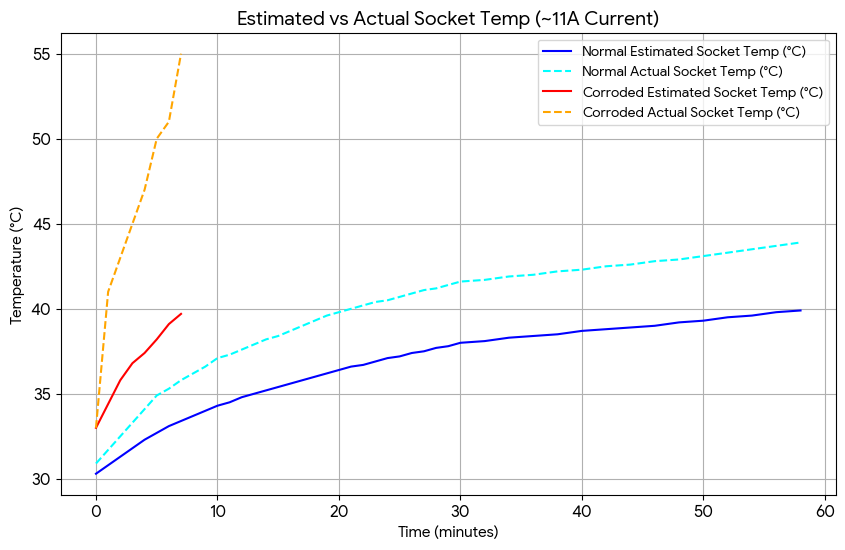
\includegraphics[height=1.65in,keepaspectratio]{figures/socket_heating_11a.png}
		\caption{Approximately 11 A}
	\end{subfigure}
	\hfill
	\begin{subfigure}[t]{0.48\linewidth}
		\centering
		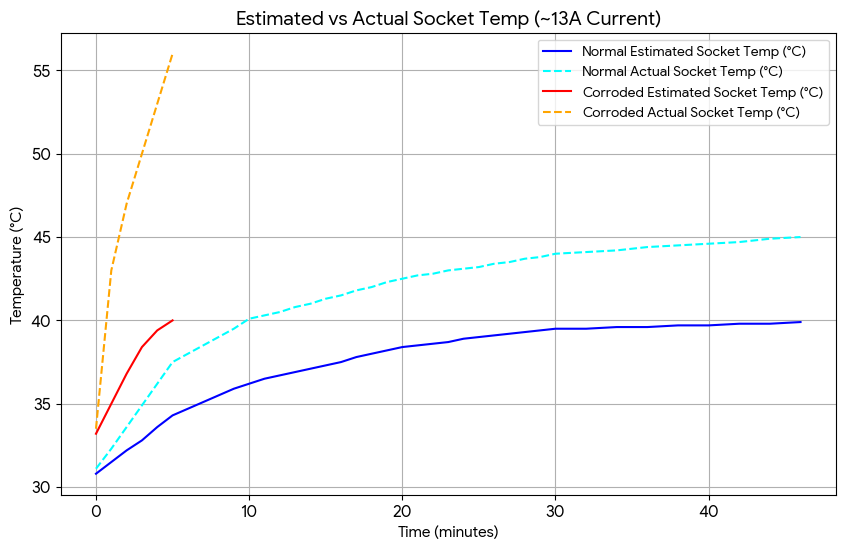
\includegraphics[height=1.65in,keepaspectratio]{figures/socket_heating_13a.png}
		\caption{Approximately 13 A}
	\end{subfigure}
	\caption{Representative socket-heating protection-validation trends under normal and corroded contacts.}
	\label{fig:socket-heating-trends}
\end{figure*}

For series-arc detection, the complete deployed system detected 96 of 100 arc trials and produced one trip during 100 normal trials. Recognized loads accounted for 49 detected arcs, one missed arc, 50 correct normal outcomes, and no false trip. Unrecognized loads accounted for 47 detected arcs, three missed arcs, 49 correct normal outcomes, and one false trip. The residual errors therefore came mainly from more difficult or unrecognized load behavior, as shown in Table~\ref{tab:arc-performance}.

\begin{table}[!b]
  	\centering\footnotesize\sffamily
  	\caption{Trial-level series-arc performance by load setup.}
  	\begin{tableminipage}{\linewidth}
    	\begin{tabularx}{\linewidth}{p{0.26\linewidth}YYYY}
			\toprule
            Load setup & Accuracy & Prec. & Recall & F1-score \\
	    	\midrule
            Recognized & 99.00\% & 100.00\% & 98.00\% & 98.99\% \\
            Unrecognized & 96.00\% & 97.92\% & 94.00\% & 95.92\% \\
            All tested loads & 97.50\% & 98.97\% & 96.00\% & 97.46\% \\
            \bottomrule
    	\end{tabularx}
        \label{tab:arc-performance}
  	\end{tableminipage}
\end{table}

The exported Random Forest report provided a second view before full relay-level interpretation. In 10,268 held-out feature frames, the report contained 10,173 true negatives, 5 false positives, 25 false negatives, and 65 true positives. The corresponding frame-level accuracy was 99.7078\%, precision was 92.8571\%, recall was 72.2222\%, and F1-score was 81.25\%. These values were lower than the trial-level relay metrics because the report evaluated individual feature frames before persistence logic and trial-level interpretation.

\section{DISCUSSION}

The results support the feasibility of a local protective layer that acts closer to the plug-socket interface than panel-level protection. Overload behavior was intentionally conservative: the device warned for heavy load combinations and tripped only after sustained current stress accumulated. This behavior is suitable for a prototype intended to distinguish short transients from thermal overload stress.

The socket-heating result is the strongest justification for localized thermal supervision. Reduced contact force, poor plug-receptacle contact, glowing contact, and arc tracking are established contributors to electrical fire risk \citep{Hadziefendic2018ReducedTorque,Hadziefendic2019PoorContacts,Zhang2023GlowingContact,Okamoto2022ArcTracking}. The prototype reproduced the practical concern in a controlled setting: degraded contacts heated faster and the hotter terminal region exceeded the device-side thermal estimate. The device-side thermistor is therefore useful as a protection-facing proxy, but it should not be interpreted as the true internal contact temperature.

The arc-detection results are encouraging but bounded. Current fluctuation, low-current behavior, zero-region features, and spectral disturbance are established indicators for series-arc detection \citep{Zhao2022SeriesArc,Gong2022SeriesArc,Chen2024LightweightArc,Qi2024SeriesArcELM}. The prototype converted these ideas into an embedded TinyML workflow by combining selected waveform features with load-family context. However, the remaining missed arcs and the single false trip occurred mainly in more difficult load behavior, which is consistent with load-monitoring literature showing that appliance current signatures vary across load families and models \citep{Medico2020PLAID,Shareef2023NILM}.

Several limitations remain. The experiments were controlled and prototype-scale, not long-term household field trials. The load and fault set did not cover all appliances, contact materials, electrode gaps, wiring conditions, nuisance transients, or ambient conditions. The thermal estimator used a non-intrusive sensor location and can under-read internal hotspots. The model also depends on dataset diversity; expanding normal, transient, nuisance, and arc examples is necessary before claims of consumer-ready reliability or standards equivalence can be made. The device should therefore be viewed as a complementary protective platform rather than an AFCI-equivalent product.

\section{CONCLUSIONS}

This study demonstrated the controlled-laboratory feasibility of a TinyML-enabled smart plug for local intervention against sustained overload, series-arc, and degraded-contact heating risks. The prototype combined custom sensing hardware, current-waveform acquisition, socket-temperature estimation, feature engineering, load-context inference, Random Forest arc classification, deterministic overload and heating protection, and relay-based local disconnection. The strongest results were sustained-overload tripping after 61.3 s in the highest-current case, faster and hotter degraded-socket heating under comparable load, and 97.50\% trial-level series-arc accuracy across 200 arc and normal outcomes.

Future work should expand the arc and nuisance-load datasets, validate the thermal estimator across additional sockets and contact materials, improve sensor placement or contact-temperature modeling, and conduct longer-term household-style trials. The prototype is best interpreted as a complementary local protection layer, not a device that fully prevents all electrical fires.

\section*{ACKNOWLEDGMENTS}

The authors acknowledge Ateneo de Naga University and the College of Science, Engineering and Architecture for academic support and laboratory resources during the research.

\section*{AUTHORS' CONTRIBUTIONS}

FMP led the design, implementation, data analysis, TinyML workflow, validation, and manuscript preparation. JML designed the ACS37035 current-sensor module, helped initialize the first test bench, assisted component procurement, contributed to data collection, and provided formatting and technical inputs. AAA refined the test bench, contributed to data collection, and provided manuscript inputs. RDS supervised the research direction, methodology, and manuscript review. All authors read and approved the final manuscript.

\section*{COMPETING INTERESTS}

The authors declare no competing interests.

\nolinenumbers
\bibliography{references/references}

\atColsEnd{\vfill}

\end{document}
